\chapter{Methodology}
%\todo{Data Preprocessing}
%\todo{- talk about all the data preprocessings steps. PCA, and collect the the top 10 PCs and how that is define, show the table.}
%\todo{Implementation}
%\todo{- defien the trainng and testing data}
%\todo{- Explain the cording process and any complications}
%\todo{Refinement}
%\todo{- Explain how the process improved. show the initial with someother activation function with bad outputs and bad loss funcitons. show some bad initial results.}

Initial Threshold Crossing Events (TCE) catalog contains 237 attributes. Each of these attributes has different strengths when it comes to classifying the ephemerides. For us to develop and train a proper network model to classify Kepler dataset, we need to understand the variables in the catalog carefully. As describe in the previous section,  there are many variables in the dataset that needed to be in the final input dataset of the network; however, dependencies between variables and non-significant variables need to remove from the dataset of entry in order to increase the performance of the network. To achieve high performance, we reducing the dataset using Principal Component Analysis and selecting top components to use as features. 

\section{TCE Catalog data cleanup}


Once download the TCE catalog from the NASAs data archives, I do process the dataset and clean them up. The initial raw data is in comma separated format where the comments are included at the beginning of the file with the descriptions of the columns and their units. I separated these comment section and created a separate data file with each row consists of a column name, its description and given units. This information later uses as a reference to get the description of the TCE catalog variables. The data values are loaded to a \emph{DataFrame}(using python \emph{pandas} module). There are some handful of columns are not completed in this dataset and left empty (and with zero value), these columns are dropped since these \emph{nul}l and zero values do not play any role.

Once we reduce these null values, we standardize the all the values in the \emph{DataFrame}. Standardization of the data is done using the \texttt{StandardScaler} function in the \texttt{sklearn.preprocessing} module. Standardization of datasets is a general requirement for many machine learning estimators. Unstandardized data might behave poorly if the individual features do not more or less look like standard normally distributed data: Gaussian with zero mean and unit variance. These standardized data has been saved as a comma separated dataset into a file. 

\section{Apply PCA to TCE Catalog }
Next step is to perform Principal Component Analysis (PCA) on the standardized TCE dataset. Standardized data set loaded from the file and apply the Principal Components Analysis using sklearn.decomposition PCA method. All the results of the PCA have been saved to a file comma separated files.

\subsection{Data Analysis}
I examine eigenvalues of PCA to determine how many principal components should be considered. Table \ref{tbl:pca} show the Eigenvalues, its proportions and the cumulative values of principal components.  The proportion of variance calculated by Equation \ref{eq:Pi}. The first eigenvalue explains about $19\%$ of the variance. The cumulative percentage calculated by adding the successive proportions of variations explained to obtain the running total. For instance the $19.00\% + 13.60\%$ equate to $32.60\%$ for the second eigenvalue ($\lambda_2$). This means the first two eigenvalues represent $32.60\%$ variances of the dataset. To determine the number of principal components we need to use, we can plot the Cumulative variance vs the principal components as shown in the figure \ref{fig:pca_cumulative}. The Cumulative variance will add up to $100\%$, this mean, the all the PCs contain the $100\%$of the variance of the dataset as it should be. It is apparent from the plot when we reach the $20^{th}$ component we almost capture total variance of the dataset. From the table \ref{tbl:pca} we can see $20^{th}$ PC has the $94.57\%$ of the variance captured. Using this method, I have experimented with the number of PCs need to include as the input the neural network to produce proper results. 


\begin{equation}
P_i = \frac{\lambda_i}{\sum_{i=1}^{n} \lambda_i}
\label{eq:Pi}
\end{equation}

\begin{equation}
C_i = P_i  + C_{i-1}
\label{eq:Ci}
\end{equation}


\begin{table}[]
%\centering
\begin{tabular}{|l|l|l|l|}
\hline
\textbf{Component} & \textbf{Eigenvalue ($\lambda_i$)} & \textbf{Proportion $\%$ ($P_i$)} & \textbf{Cumulative $\%$} ($C_i$) \\ \hline
PC1 & 7.4114 & 19.00 & 19.00 \\ \hline
PC2 & 5.30315 & 13.60 & 32.60 \\ \hline
PC3 & 3.30398 & 8.47 & 41.07 \\ \hline
PC4 & 2.84707 & 7.30 & 48.37 \\ \hline
PC5 & 2.57537 & 6.60 & 54.97 \\ \hline
PC6 & 2.17668 & 5.58 & 60.55 \\ \hline
PC7 & 1.63915 & 4.20 & 64.75 \\ \hline
PC8 & 1.43721 & 3.69 & 68.44 \\ \hline
PC9 & 1.33558 & 3.42 & 71.86 \\ \hline
PC10 & 1.16966 & 3.00 & 74.86 \\ \hline
PC11 & 1.09168 & 2.80 & 77.66 \\ \hline
PC12 & 1.0003 & 2.56 & 80.22 \\ \hline
PC13 & 0.901048 & 2.31 & 82.53 \\ \hline
PC14 & 0.836118 & 2.14 & 84.67 \\ \hline
PC15 & 0.81133 & 2.08 & 86.75 \\ \hline
PC16 & 0.7114 & 1.82 & 88.57 \\ \hline
PC17 & 0.678007 & 1.74 & 90.31 \\ \hline
PC18 & 0.602895 & 1.55 & 91.86 \\ \hline
PC19 & 0.584217 & 1.50 & 93.36 \\ \hline
PC20 & 0.472781 & 1.21 & 94.57 \\ \hline
PC21 & 0.447496 & 1.15 & 95.72 \\ \hline
PC22 & 0.380196 & 0.97 & 96.69 \\ \hline
PC23 & 0.315781 & 0.81 & 97.50 \\ \hline
PC24 & 0.234446 & 0.60 & 98.10 \\ \hline
PC25 & 0.183911 & 0.47 & 98.57 \\ \hline
PC26 & 0.153009 & 0.39 & 98.96 \\ \hline
PC27 & 0.12802 & 0.33 & 99.29 \\ \hline
PC28 & 0.123365 & 0.32 & 99.61 \\ \hline
PC29 & 0.0969348 & 0.25 & 99.86 \\ \hline
PC30 & 0.0174445 & 0.04 & 99.90 \\ \hline
PC31 & 0.0152885 & 0.04 & 99.94 \\ \hline
\end{tabular}
\caption{Eigenvalues, and the proportion of variation produced by the principal components (Only first 31 components are listed).}
\label{tbl:pca}
\end{table}

\begin{figure}[!h]
\begin{center}
        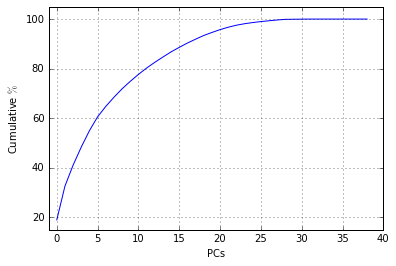
\includegraphics[width=0.4\textheight]{img/pca_cumulative.png}
        \caption{Cumulative $\%$}  \label{fig:pca_cumulative}
\end{center}
\end{figure}

\begin{table}
\begin{center}
        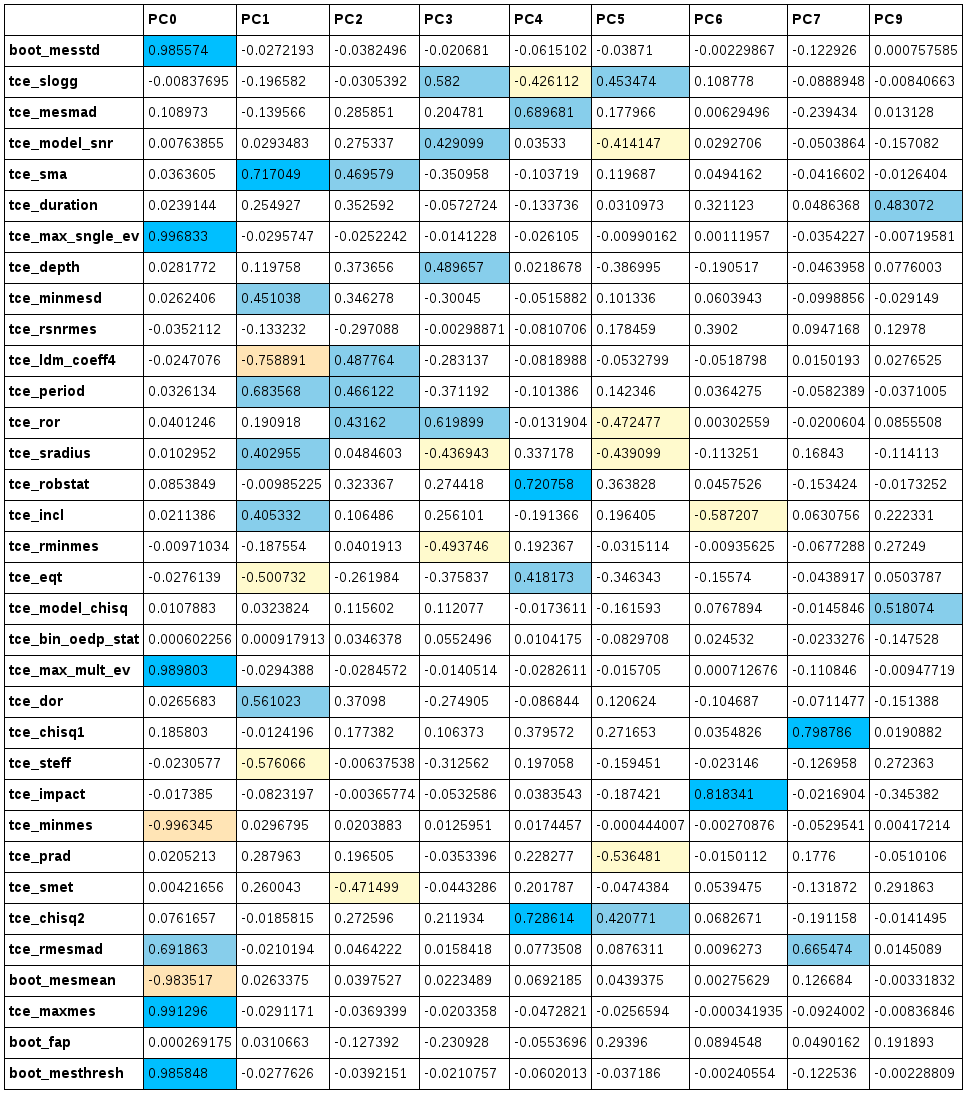
\includegraphics[width=0.75\textheight]{img/pc_corr.png}
        \caption{Correlation between Principal Components and Variables}  \label{fig:pc_corr}
\end{center}
\end{table}


Furthermore, we can interpret each of the principal components using the correlations between the original data for each variable and principal components. The correlations can be obtain using correlations procedure. The Table \ref{fig:pc_corr} show the correlation coefficients between PCs (first 10) and original variables (rows). Due to the standardization, all PCs will have mean of zero. Standard Deviation is also given for each of the components and these will be the square root of the eigenvalue. The interpretation of principal components is based on the variables are most strongly correlated with each component, i.e, which of these number are large in magnitude, the farthest from zero in either positive or negative direction. Table \ref{fig:pc_corr} show the correlation values greater than $0.7$ in one color (dark blue) and between $0.4$ and $0.7$ (lighter blue) in one color and the negative correlations using other colors (dark yellow and lighter yellow). These interpretation allow us to have a clear understanding which variables are correlated with which principal component. However, to continue with the calculated principal components as input to the neural network, this knowledge is not nessasary, this is purely to understand the dataset in depth to interpret physics behind it.

\section{Training and Testing Data}
Before we train the neural network with the transformed TCE dataset, we ned to split the data into two sections: training and testing data. Training the network with one dataset and testing with another dataset allow us to avoid overfitting. To split the data into these sets, we are using the \texttt{scikit-learn} a random \texttt{split train\_test\_split} helper function. We can tell this method what ratio it should need to split the data. Once we do that, the method split the data according to the ratio randomly selecting a number of data records as training and testing. The helper method takes the TCE catalog data and the labels as parameters. 

\section{Training the Neural Network}
Once the data has been cleanup, standardized, transform using Principal component analysis and split into testing and training data sets, next step is to train a neural network. We create a Multi-layered perceptron (MLP) that trains using backpropagation network using  \texttt{MLPClassifier} in  \texttt{sklearn.neural\_network} package. When creating the MLP, there are several parameters we need to define. These parameters are picked after analyzing the behavior of them with the dataset. 

\subsection{Activation Function}
There are several built-in activation functions are in the scikit learn. Primarily these activations functions are divided into two different categories for two different output layers: non-linear and linear or softmax layers.  We compute the loss function for activation functions where we can see the how the loss function behave. List of activation functions:

\begin{itemize}
\item \emph{Identity}: this is a linear function without changing the input, this is useful to implement linear bottleneck, Equation \ref{eq:identity}
\begin{equation}
f(x) = x
\label{eq:identity}
\end{equation}

\item \emph{Logistic}: This is a logistic sigmoid function, Equation \ref{eq:logistic}
\begin{equation}
f(x) = \frac{1}{(1+e^{-x})}
\label{eq:logistic}
\end{equation}

\item \emph{Relu}: This is a rectified linear unit function, Equation  \ref{eq:relu}
\begin{equation}
f(x) = max(0, x)
\label{eq:relu}
\end{equation}

\item \emph{tanh}: The hyperbolic tan function, Equation  \ref{eq:tanh}
\begin{equation}
f(x) = tanh(x)
\label{eq:tanh}
\end{equation}

 
\begin{figure}[!h]
\begin{center}
        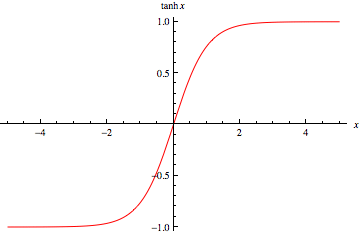
\includegraphics[width=0.3\textheight]{img/tanh.png}
        \caption{\emph{tanh} function}  \label{fig:tanh}
\end{center}
\end{figure}

After some experiments and the nature of the \emph{tanh} function (Figure \ref{fig:tanh}), we have picked the \emph{tanh} function as the activation function for the network.

\end{itemize}


\subsubsection{Loss Function}

Log loss is also known as logistic regression loss or cross-entropy loss is defined on probability estimate. Usual application for logistic regression is a binary classification, however, it is easy to extend this to a multiclass case \cite{bishop2006pattern}, Equation \ref{eq:logloss}. 
\begin{equation}
L_{log}(Y, P) = -logPr(Y|P) = -\frac{1}{N}\sum_{i=0}^{N-1}\sum_{k=0}^{K-1}y_{i, k}log p_{i, k}
\label{eq:logloss}
\end{equation}


\begin{figure}[!h]
\begin{center}
        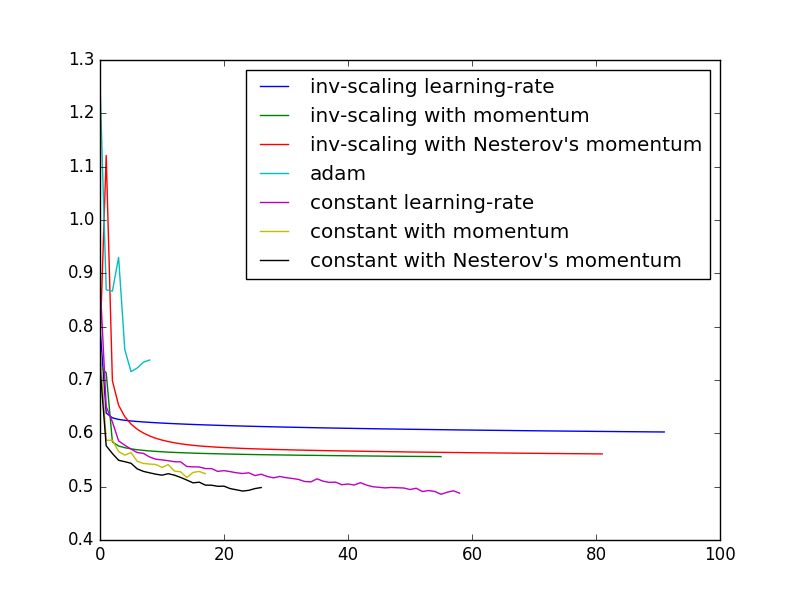
\includegraphics[width=0.5\textheight]{img/activation_functions_1.png}
        \caption{Loss function with some learning rate methods. x-axis: number of iterations. y-axis: loss function value}  \label{fig:loss_functions}
\end{center}
\end{figure}


\subsection{Learning Rate - $\eta$}
It was appetent the behavior of the network with the activation function being the tanh highly depend on the learning rate. Learning rate ($\eta$) is explained using the equation \ref{eq:gd} in the section \ref{sec:mlp}. scikit lean allow to configure the neural network with several different learning rate methods: 

\begin{itemize}
\item \emph{constant}: A constant learning rate, the value is taken as an integer value
\item \emph{invscaling}: Gradually decreases the learning rate at each time step $t$ using an inverse scaling exponent of \emph{power\_t}.
\item \emph{adaptive}: Keep the learning rate constant as long as training loss keeps decreasing. Each time two consecutive epochs fail to decrease training loss by at least \emph{tol} ($=0.0001$), or fail to increase validation score by at least an amount that defined as tol, or if \emph{early\_stopping} is \emph{on}, the current learning rate is divided by 5.
\end{itemize}

Figure \ref{fig:loss_functions} show the behavior of the loss function for several learning rates we have experimented with the dataset. The goal is to bring the loss function to close to zero that indicates the convergence of the network. The x-axis shows the number of iterations. 

\begin{figure}[!h]
\begin{center}
        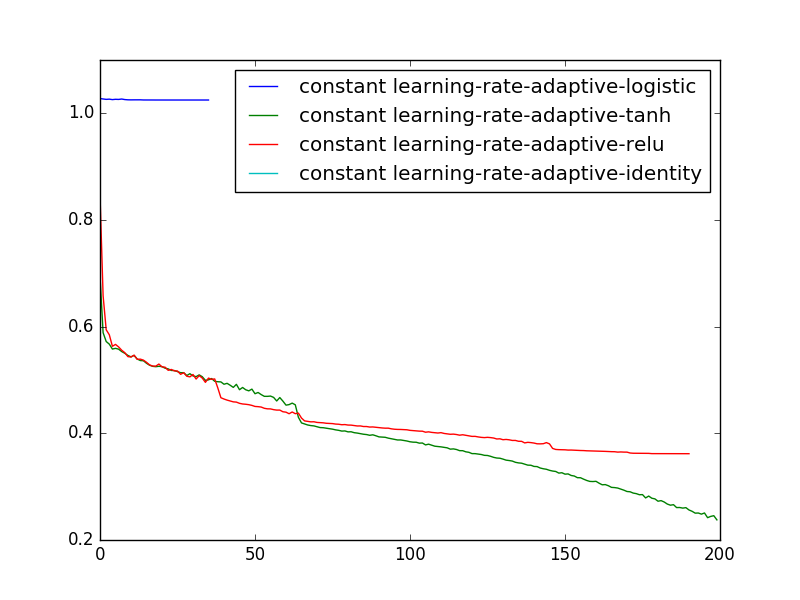
\includegraphics[width=0.5\textheight]{img/constant_learning_rate.png}
        \caption{Loss function with constant learning rate with different activation methods. x-axis: number of iterations. y-axis: loss function value}  \label{fig:loss_functions_2}
\end{center}
\end{figure}

\begin{figure}[!h]
\begin{center}
        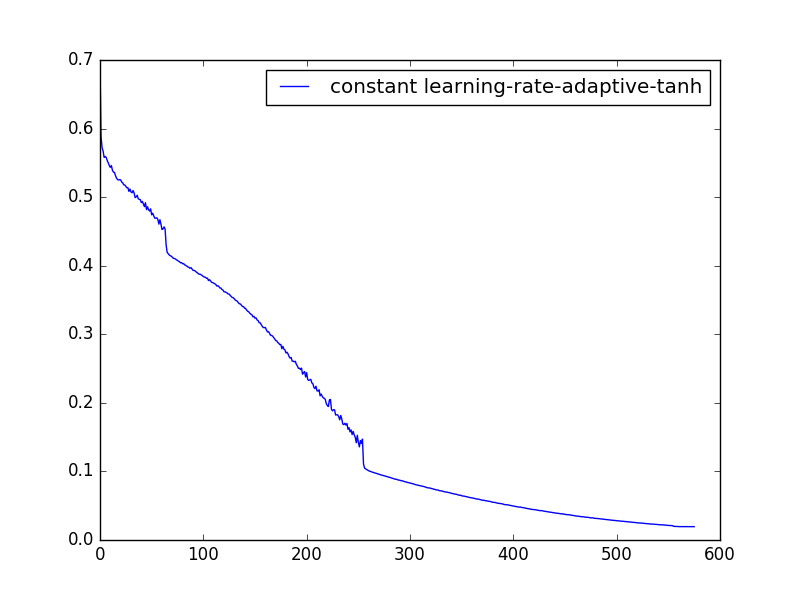
\includegraphics[width=0.5\textheight]{img/constant_learning_rate_final.png}
        \caption{Loss function with constant adaptive learning rate with \emph{tanh} activation method converge the network. x-axis: number of iterations. y-axis: loss function value}  \label{fig:loss_functions_3}
\end{center}
\end{figure}

After seeing the constant learning rate is keep reducing the loss function, I have experimented with the constant learning rate  (set for 0.2) with different activation functions. Figure \ref{fig:loss_functions_2} show some results of this work. It is clear that constant learning rate with adaptive method for the learning rate and \emph{tanh} for the activation function is quite impressively kept reducing the loss function. I have tested with this particular combination further and the result is shown in the figure \ref{fig:loss_functions_3}. Constant learning rate with adaptive method combine with the \emph{tanh} activation method converge the network close to 600 iterations, thus we are settling with this configuration for to train the neural network with TCE catalog data. 

MLPClassifier trains iteratively since each time step the partial derivative of the loss function with respect to the model parameters are computed to update the parameters. Once we fix the parameters of the network, we train the network with training dataset we pick out of the entire catalog. This training process took about 15 minutes to complete, once this complete I save the trained classifier as a python \texttt{pickle} object where the program can load the train network to test the test dataset without keep training every single time. The program config file let you pick a name for the train network where the program looks for a \texttt{pickle} file under that name at the beginning of the program to load. 
